% THIS IS SIGPROC-SP.TEX - VERSION 3.1
% WORKS WITH V3.2SP OF ACM_PROC_ARTICLE-SP.CLS
% APRIL 2009
%
% It is an example file showing how to use the 'acm_proc_article-sp.cls' V3.2SP
% LaTeX2e document class file for Conference Proceedings submissions.
% ----------------------------------------------------------------------------------------------------------------
% This .tex file (and associated .cls V3.2SP) *DOES NOT* produce:
%       1) The Permission Statement
%       2) The Conference (location) Info information
%       3) The Copyright Line with ACM data
%       4) Page numbering
% ---------------------------------------------------------------------------------------------------------------
% It is an example which *does* use the .bib file (from which the .bbl file
% is produced).
% REMEMBER HOWEVER: After having produced the .bbl file,
% and prior to final submission,
% you need to 'insert'  your .bbl file into your source .tex file so as to provide
% ONE 'self-contained' source file.
%
% Questions regarding SIGS should be sent to
% Adrienne Griscti ---> griscti@acm.org
%
% Questions/suggestions regarding the guidelines, .tex and .cls files, etc. to
% Gerald Murray ---> murray@hq.acm.org
%
% For tracking purposes - this is V3.1SP - APRIL 2009

\documentclass{acm_proc_article-sp}
\usepackage{array}
\newcolumntype{L}[1]{>{\raggedright\let\newline\\\arraybackslash\hspace{0pt}}m{#1}}
\newcolumntype{C}[1]{>{\centering\let\newline\\\arraybackslash\hspace{0pt}}m{#1}}
\newcolumntype{R}[1]{>{\raggedleft\let\newline\\\arraybackslash\hspace{0pt}}m{#1}}

\begin{document}

\title{Predicting Daily Active Users for Match-3 Mobile Games}

%
% You need the command \numberofauthors to handle the 'placement
% and alignment' of the authors beneath the title.
%
% For aesthetic reasons, we recommend 'three authors at a time'
% i.e. three 'name/affiliation blocks' be placed beneath the title.
%
% NOTE: You are NOT restricted in how many 'rows' of
% "name/affiliations" may appear. We just ask that you restrict
% the number of 'columns' to three.
%
% Because of the available 'opening page real-estate'
% we ask you to refrain from putting more than six authors
% (two rows with three columns) beneath the article title.
% More than six makes the first-page appear very cluttered indeed.
%
% Use the \alignauthor commands to handle the names
% and affiliations for an 'aesthetic maximum' of six authors.
% Add names, affiliations, addresses for
% the seventh etc. author(s) as the argument for the
% \additionalauthors command.
% These 'additional authors' will be output/set for you
% without further effort on your part as the last section in
% the body of your article BEFORE References or any Appendices.

\numberofauthors{3} %  in this sample file, there are a *total*
% of EIGHT authors. SIX appear on the 'first-page' (for formatting
% reasons) and the remaining two appear in the \additionalauthors section.
%
\author{
% You can go ahead and credit any number of authors here,
% e.g. one 'row of three' or two rows (consisting of one row of three
% and a second row of one, two or three).
%
% The command \alignauthor (no curly braces needed) should
% precede each author name, affiliation/snail-mail address and
% e-mail address. Additionally, tag each line of
% affiliation/address with \affaddr, and tag the
% e-mail address with \email.
%
% 1st. author
\alignauthor
Neil Patrick Del Gallego \\
       \affaddr{College of Computer Studies}\\
       \affaddr{De La Salle University - Manila}\\
       \email{neil.dg@pocketplaylab.com}
% 2nd. author
\alignauthor
Arvin Corpuz \\
       \affaddr{College of Computer Studies}\\
       \affaddr{De La Salle University - Manila}\\
       \email{2nd email}
% 3rd. author
\alignauthor 
Oliver Bob Urag \\
       \affaddr{College of Computer Studies}\\
       \affaddr{De La Salle University - Manila}\\
       \email{3rd email}
}

\maketitle
\begin{abstract}
We present in this paper a technique to attempt to predict the amount of daily active users for a match-3 mobile game by considering several factors that drives a game's social virality. The data was extracted from the performance of two match-3 mobile games by Playlab Inc., Jungle Cubes and Dragon Cubes. In this paper, we describe our experiments on these two games and the outcomes of the prediction model extracted.
\end{abstract}

\keywords{Data Mining, Classification, Regression, Daily Active Users, Mobile Games, Free-to-play, Retention.}

% Contains the introduction
%
%
%
\section{INTRODUCTION}
Free-to-play mobile games follow a common business model. It is a necessity that these games have a healthy community to drive the virality of the game. One of the key measures for determining the success of a mobile game is by using Daily Active Users (DAU) as a metric. This refers to the total amount of unique users who spent considerable time in the game given a certain date. This refers to the "stickiness" of the application. A high value for DAU indicates that there is much activity and demand for the mobile game. It is essential for game development companies that develop mobile games that follows a free-to-play model, to keep the DAU value as high as possible.  This paper attempts to predict DAU value for two commercial match-3 mobile games, Jungle Cubes and Dragon Cubes, that are currently owned by Playlab Inc.

Companies that follow a free-to-play business model use various analytics tools to track user's behavior and events triggered in their applications. In this study, Playlab Inc., uses Flurry Analytics and Google Play Developer Console to collect user data. One of the attributes capable of being tracked is the DAU.

In this study, we present a hypothesis that the DAU value is driven by other attributes or events that causes a user to use the application (or in this case, play for a considerable time) extensively. Such attributes considered are discussed in the succeeding sections.

Business decisions for a mobile game are executed when there is sufficient user data collected. One of the major problems encountered by companies such as Playlab Inc., is that major releases for the game don't immediately provide significant user data. It would be appropriate to provide a forecasting technique to determine if there would be a significant user activity on succeeding days. In a practical scenario, this paper aims to answer the question; given a certain day with these collected attributes, how high will the DAU value be X days after? In our experiments, we specifically attempt to predict the Daily Active Users value at Day 7.

% Contains the significance of the study and related literature.
%
%
%
\section{SIGNIFICANCE OF THE STUDY}
Behavioral analytics has recently emerged as a practice for commercial game development. These also relates to technological advancements brought about by mobile devices that enable developers to gather more significant data through the use of commercial analytics.

There is a significant increase on the number of games that are shifting to the free-to-play (F2P) model and this study are one of the few instances wherein commercial game dataset are used for academic research. Findings will be beneficial for game companies that strictly complies with the F2P model. In specific, those who greatly rely on high user activity for their games will strongly find this paper beneficial for their business decisions.

We present a novel approach on how analysts or developers may attempt to predict the DAU value on a practical scenario, based from the formula given by our prediction model. We also attempt to define features that are highly important based from our analysis of attributes on our dataset and as supported by other similar study as seen in \cite{ref:predicting_player_churn}.

In this manner, we present the following contributions in this paper:
We formally define from related study, as well as our findings,  the attributes that affects the DAU value.
We attempt to create several prediction models for the DAU value using machine learning techniques and explain its significance on a practical setting.
We present a simple method on how one can predict the DAU value
This paper are one of the few research study that uses dataset from commercial games which is otherwise, confidential and unavailable for academic research.
Despite a small number of installs for both games, Jungle Cubes have very strongly correlated attributes against DAU, which make the dataset significant. We present this in detail in the succeeding sections.

\subsection{Related Work}
Using game analytics for research purposes has recently been pursued around 2012.  Analysis of user behavior in digital games has become a fundamental practice for game companies. It is also open for numerous research opportunities due to its complex nature of modelling users while also taking into consideration the elements of the game. Thus, datasets concerning player behavior can be exceptionally complex like seen in World of Warcraft, a famous MMORPG (Massively Multiplayer Online Role-Playing Game), which has lead a team of researchers attempt to cluster players based from behavioral telemetry \cite{ref:player_clustering_wow}. They applied numerous unsupervised learning methods to discover clusters of "player groups" based from their playtime data and their levelling pace.

\subsubsection{Determining How Players Lose Interest}
A study on action and shooter games released on Playstation 3, that uses player behavior dataset, have been used to discover how players lose interest in playing a game \cite{ref:how_players_lose_interest}. The dataset presented in their research paper were extracted from two single-player games (Just Cause 2, Tomb Raider: Underworld) and three multi-player games (Battlefield Bad Company 2, Medal of Honor, Crysis 2).  All datasets have been sampled using simple random sampling or extraction of data on a timeline where player activities are high or the game was newly released.

The interest of playing a game cannot be measured directly but can be inferred from observable data as mentioned by \cite{ref:how_players_lose_interest}. In reality, a player's urge to play a game is influenced by several factors that appears as unforeseeable events to the analysts involved. This ranges from variance in playing schedules, personal satisfaction, release of new game content, or new games that competes with the player's attention. Using these consideration as mentioned by \cite{ref:how_players_lose_interest}, they modeled the player's interest in playing a game as a random process. That is, at any given time, a player's interest is a random quantity that may or may not depend on previous values and future values cannot be predicted exactly. Thus, they have restricted their mathematical models to random process models; the Gamma distribution, Weibull distribution, Inverse Gaussian distribution, and Log-normal distribution.

Of all five games analyzed, researchers deduced that the total playing times follows the Weibull distribution. Following the Weibull model, it gives a good benchmark for gaming companies to determine how a player's playtime even before the game has been released.

\subsubsection{Predicting Churn Rate}
There is an existing research work that is highly related to our methodology. Researchers attempted to predict the Churn Rate of commercial mobile games which also uses some attributes we use for this study \cite{ref:predicting_player_churn}. In their study, they threat the churn value as a binary classification task, a player is labelled as \textbf{churned} or \textbf{returning}. Given a specified \textit{cutoff date}, the player will be labelled as \textbf{churned} or \textbf{returning} based from two formal problems defined in their study.

They described problem \textbf{P1} to be more straightforward. Given a cutoff date, players who did not return after the cutoff date are immediately considered as churners. The green dots in \ref{fig:churn_figure} are considered as \textbf{churners} while the red dots are players who managed to return after the specified cutoff date. This formal definition of churn is harsh and not useful for real-world applications. Problem \textbf{P2} is more relaxed. Given a grace period after the specified cutoff date, if players return during this period, they are considered as "about to churn" wherein their engagement to the game is already low. These are the players who are likely to quit soon and knowing how much players are inside this grace period aids gaming companies on potentially rescuing these players to get back to the game. In \ref{fig:churn_figure}, the first two green dots refer to players already churned while the third green dot inside the grace period is flagged as "about to churn." The red dot is a player who managed to return to the game after the grace period.

Figure \ref{fig:churn_figure} shows an illustration of formal problem \textbf{P1} and problem \textbf{P2}.

\begin{figure*}[h]
\centering
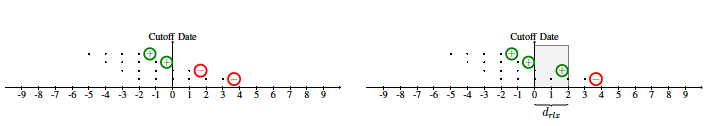
\includegraphics[scale=0.6]{figures/churn.png}
\caption{Formal problems defined as \textbf{P1} and \textbf{P2} described by \cite{ref:predicting_player_churn}. \textbf{P1} defines users as churners if they do not return after the specified cutoff date. In \textbf{P2}, players are given a grace period after the cutoff date. If players did not return after the specified grace period, they are considered as churners. }
\label{fig:churn_figure}
\end{figure*}


\begin{itemize}
\item Feature Selection \\
Attributes were universal and game-content independent. The following attributes stood out based from their feature selection tests and obvious observations that affect churning behavior; \textbf{Number of Sessions}, \textbf{Number of Days}, \textbf{Current Absence Time}, \textbf{Playtime per Session}, and \textbf{Average Time Between Sessions} and \textbf{Predefined Spending Category}. Some of these attributes are observed in our study.

\item Experiments and Results \\
In their research work, the  most accurate classifier is the decision tree, among other different classifiers; neural networks, logistic regression, and naive bayes. F1-score goes as high as 0.916 for the decision tree model. 
\end{itemize}




\section{Dataset and Information About Attributes}
This section contains an overview of the dataset used for this paper. The manner of extraction is also discussed in this section. Attributes are defined as well. 

There are two datasets available for research and both are considered for the empirical study. The DNC Dataset and the JNC Dataset. Both datasets have been compiled and retrieved from Flurry Analytics, a commercial analytics tool used by Playlab Inc to track user's behavior on their commercial mobile games. Some attributes were retrieved from Google Play Developer Console such as user's ratings and daily crash reports. The DNC dataset refers to the Dragon Cubes game while the JNC dataset refers to the Jungle Cubes game. Both dataset are restricted to Android platforms only.

\ref{table:dataset_overview} shows the overview of the datasets used for the study.

\begin{table}
\centering
\caption{Overview of Dataset Used}
\label{table:dataset_overview}
\begin{tabular}{| C{2cm} | C{1cm} | C{1cm} | C{1cm} | C{1.5cm} |}
\hline 
Dataset Filename & Game Title & Total Downloads & Overall Rating & Timeline of Dataset \\ 
\hline 
DNC Dataset Android 0511-0911 & Dragon Cubes & 50,000 - 100,000 & 4.2 out of 5 & May 11, 2015 - September 11, 2015 \\ 
\hline 
JNC Dataset Android 0511-0911 & Jungle Cubes & 100,000 - 500,000 & 4.3 out of 5 & May 11, 2015 - September 11, 2015 \\ 
\hline 
\end{tabular}
\end{table} 

Both datasets spans on a similar timeline, that is May 11 - September 11,2015. A span of four months have been deemed sufficient for analysis and increasing the timespan no longer yields better results.

\section{Attribute Information}
This section discusses the attributes used for this study.  \ref{table:dataset_attributes} contains the definition of attributes found in the dataset. These attributes have been gathered and selected from Flurry Analytics and Google Play Developer Console. 

The initial selection of dataset has been manually performed by the researchers which they have deemed sufficient for analysis and have potential impact to the DAU value. On the succeeding section, we analyzed each variable and their correlation values to determine which variables have high relationship with the DAU value.

\begin{itemize}
\item Install Date - Each instance in the dataset is organized by install date. This refers to the gregorian calendar date wherein an application is installed.
\item Cohort Size - Refers to the total amount of users who have installed the application on the given install date.
\item Day X - This represents the retention of the application given a certain date and cohort size. Installation date becomes day 0. Retention rate is the percentage of returning users on a specified install date. For example, day 1 has 40.75\% retention and 1200 cohort size. Therefore, 40.75\% of users have managed to return on day 1 (489 users in cohort size)
\item CrashesANRDay1 - reality, crash reports come in a day after the specified install date. For example, May 11,2015 has 3 crash reports. This means that this value was only retrieved on May 12, 2015.This counts the total number of crashes and ANRs (application not responding) reports from the application. This has a negative impact for the user experience. In reality, crash reports come in a day after the specified install date. For example, May 11,2015 has 3 crash reports. This means that this value was only retrieved on May 12, 2015.
\item DailyAverageRating - This refers to the average rating by users who choose to rate the application (1 to 5, 5 being the highest) on a given date. Rating an application is not mandatory. This is a primary determination for virality. Similar to CrashesANRDay1, the tally comes in a day after the specified install date.
\item LevelPlayedEvents - Refers to the accumulated event tally that is triggered when a user plays a level on the application. This is triggered upon tap of the 'Play' button. This event is reported no matter the outcome of the level being played.
\item LevelSuccessEvents - Refers to the accumulated events that are triggered if a user successfully completes a level. This is triggered when the 'Win' screen is shown to the user.
\item LevelFailedEvents - Refers to the accumulated events that are triggered if a user fails a level. This is triggered when the 'Lose' screen is shown to the user.
\item Session - Refers to the total amount of play sessions on a given install date. A high value for session count on a given install date means that there are a lot of playthrough activity 
\item MKTExpenses - This is the total amount of marketing expenses, in USD, spent to advertise the game. Given an install date, the marketing expense normally determines the cohort size. A high marketing expense means more advertising channels have been used to target more potential users to install the game.
\item ActiveUsers - This refers to the total amount of unique users who spent considerable time in the game given a certain date. This refers to the "stickiness" of the application.This is one of the attributes essential for determining a game's success.
\item ActiveUsersDay7 - This is similar to the ActiveUsers variable but offset 7 days after the install date. This is the variable to be predicted. 
\end{itemize}

In reality, given a install date, and one would like to know how many daily active users would there be 7 days after, the following variables will be used: Cohort Size, Day 1, CrashesANRDay1, DailyAverageRating, LevelPlayedEvents, LevelSuccessEvents, LevelFailedEvents, Sessions, MKTExpenses, and ActiveUsers.

Note that some variables like DailyAverageRating and CrashesANRDay1, only becomes available a day after. In a practical scenario, one could make predictions by Day 2 since it is assumed that all variables are readily available.

%ACKNOWLEDGMENTS are optional
\section{Acknowledgments}

%
% The following two commands are all you need in the
% initial runs of your .tex file to
% produce the bibliography for the citations in your paper.
\bibliographystyle{abbrv}
\bibliography{references}  % sigproc.bib is the name of the Bibliography in this case
% You must have a proper ".bib" file
%  and remember to run:
% latex bibtex latex latex
% to resolve all references
%
% ACM needs 'a single self-contained file'!
%
%APPENDICES are optional
%\balancecolumns

% This next section command marks the start of
% Appendix B, and does not continue the present hierarchy

\end{document}
